In this section, we first formulate the problem of traffic matrix prediction under the lack of ground-truth input. 
Then, we give a brief introduction about the Long Short-Term Memory and Convolutional LSTM networks which are used in our approach. 
We summarize the major notations in the table \ref{table:notations} for quick reference.

\begin{table}[]
\begin{tabular}{|c|l|}
\hline
Notations           & Description                                                                                                                                                              \\ \hline
N                   & Set of node in the network. |N| = n.                                                                                                                                     \\ \hline
X                   & The traffic matrix at timestep j                                                                                                                                         \\ \hline
X$\sim$             & The predicted traffic matrix for timestep j                                                                                                                              \\ \hline
x                   & Traffic volume of flow (s,d) at timesteps j. x \textbackslash{}in X                                                                                                      \\ \hline
o                   & The ground-truth value of traffic volume of flow (s,d) at timestep j                                                                                                     \\ \hline
x$\sim$             & The predicted traffic volume of flow (s,d) for timestep j.                                                                                                               \\ \hline
x\textasciicircum{} & The predicted traffic volume of flow (s,d) for timestep j by backward network.                                                                                           \\ \hline
m                   & \begin{tabular}[c]{@{}l@{}}The binary variable, m = 1 indicates that the traffic volume of flow\\  (s,d) at timestep j is ground-truth value and otherwise.\end{tabular} \\ \hline
M                   & The measurement matrix at timestep j.                                                                                                                                    \\ \hline
lf                  & The forward loss                                                                                                                                                         \\ \hline
lb                  & The backward loss                                                                                                                                                        \\ \hline
w                   & The weight of flow (s,d) is calculated at current timestep t.                                                                                                            \\ \hline
\end{tabular}
\caption{My caption}
\label{my-label}
\end{table}


\subsection{Problem Description}
\label{subsec:problem_description}

\begin{figure}
\centering
		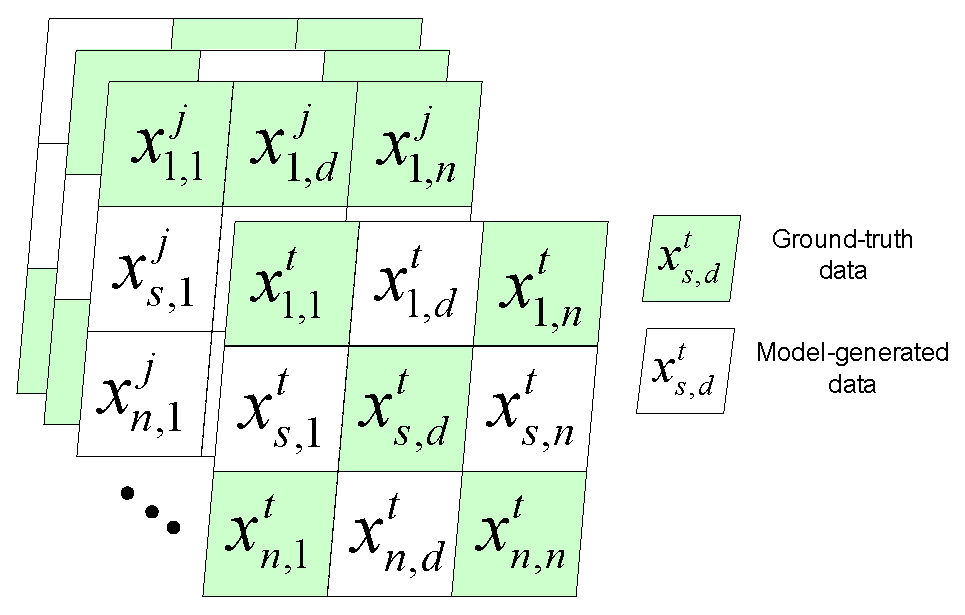
\includegraphics[width=0.65\columnwidth]{preliminaries_figs/traffic_matrices.eps}
		\caption{A sequence of $J$ previous traffic matrices including the imprecise data. \label{fig:traffic_matrices}}
\end{figure}

We suppose that the traffic monitoring and predicting tasks are executed every $\mathcal{T}$ seconds, and we call the execution timings as timesteps.
Let us denote by $t$ the current timestep.
Let $N$ be the set of nodes in the backbone network ($\left |  N \right |=n$), then the traffic matrix at timestep $j$ (denoted by $X_j$) is a $R^{n \times n}$ matrix whose each element $x_{s,d}^j$ represents the traffic volume of the flow from the origin $s$ to the destination $d$, at the timestep $j$.
To ease the presentation, throughout this paper we call a flow from $s$ to $d$ as an origin-destination flow $(s,d)$ (or $OD$ flow $(s,d)$, for short). 
Basically, the traffic matrix prediction problem is to estimate the traffic matrices of $L$ next timesteps given the previous $J$ measurements:

\begin{equation}
\begin{aligned}
&\widetilde{X}_{t+1},...,\widetilde{X}_{t+L} \\
	&\quad = \argmax_{X_{t+1},...,X_{t+L}} p(X_{t+1},...,X_{t+L} | X_{t-J+1},...,X_{t})
\end{aligned}
\end{equation}

However, in this paper, we consider the case of backbone network where obtaining all the $J$ previous traffic matrices by directly monitoring all the flows in the network is impractical. Although in recent years, the advance network architecture and management such as Software Defined Networking (SDN) [ref] and Network Function Virtualization (NFV) have enabled many alternative ways to measure the network flows information, collecting all the traffic statistics with low overhead (in terms of computational, bandwidth...) still remains as a challenging task. Therefore, to reduce the monitoring overhead, we only measure a part of the traffic flows at each timestep and use the data generated by the prediction model to fill into the traffic matrix. Thus, the traffic matrices prediction problem under highly missing ground-truth data can be formulated as follow:

\begin{equation}
\label{equation:tm_prediction_missing_data}
\begin{matrix}
x_{s,d}^{j}=\left\{\begin{matrix}
o_{s,d}^j & if m_{s,d}^j=1 \\
\widetilde{x}_{s,d}^j & otherwise
\end{matrix}\right. \\
\forall s, d \in N; j = t - J + 1,...,t \\
\begin{aligned}
\widetilde{X}_{t+1}&,...,\widetilde{X}_{t+L} \\
	& = \argmax_{X_{t+1},...,X_{t+L}} p(X_{t+1},...,X_{t+L} |  X_{t-J+1},...,X_{t})
\end{aligned}
\end{matrix}
\end{equation} where $o_{s,d}^j$ and $\widetilde{x}_{s,d}^j$ are the observed and predicted value of the $OD$ flow $(s,d)$ at timestep $j$, respectively. The binary variable $m_{s,d}^j=1$, which depends on the monitoring policy, indicates that the $OD$ flow $(s,d)$ is monitored at timestep $j$; otherwise, the value of traffic volume is filled up by the prediction result. Fig.\ref{fig:traffic_matrices} shows the sequence of $J$ previous traffic matrices which is used as the input for predicting the future traffic. The green elements are the ground-truth data obtained by monitoring the flows in the network. 

\subsection{The Long Short-Term Memory and Convolutional LSTM network for spatiotemporal sequence modeling}
\label{subsection:lstm_ConvLSTM}
\begin{figure}
\centering
		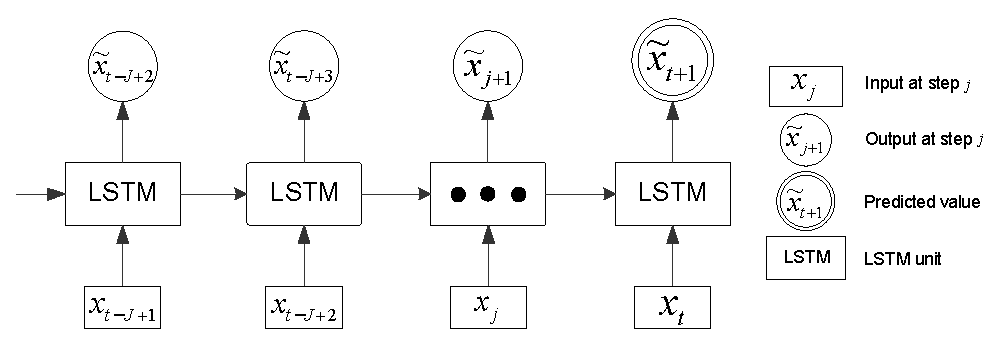
\includegraphics[width=0.9\columnwidth]{preliminaries_figs/LSTM_model.eps}
		\caption{The unfolded model of LSTM network \label{fig:LSTM_model}}
\end{figure}


Long Short-Term Memory network is a special Recurrent Neural Network which replaces the standard RNN units by the LSTM units.
LSTM network has been proved to be stable and powerful for modeling long-range dependencies in various problem domains. 
Therefore, LSTM networks are well-suited for processing and making predictions based on time series or sequence data and has been applied in many real-life sequence modeling problems. 
The unfolded model of LSTM network (Fig.\ref{fig:LSTM_model}) shows that the input is processed step-by-step and the output of previous steps are used as input for the next step. 
This architecture along with the advantages of the memory cell in the LSTM units makes the LSTM network be especially suitable for solving the time series based prediction.

However, in many problems such as precipitation nowcasting [ref] or images/videos based action prediction [ref], the sequence data contains too much redundancy for spatial data [ref]. Therefore, for more general spatiotemporal sequence forecasting problems, authors in [ref] have proposed an extension of LSTM called ConvLSTM. The ConvLSTM layer has convolutional structures in both the input-to-state and state-to-state transitions which can exploit both temporal and spatial features of the input sequence. Fig.\ref{fig:ConvLSTM_model} shows the inner structure of ConvLSTM network where the inputs $X_t$ are 3D tensor, for example $X_t$ can be a $32 \times 32 \times 3$ image in which the last dimension represents the colors of the images (RGB). The key equations of ConvLSTM are shown in equation (\ref{equation:convlstm}) where $i_t, f_t, o_t$ are the input, forget, output gate, $C_t, H_t$ are the cell and final state of the LSTM unit. The $*$ denotes the convolution operator and $\circ$ denotes the Hadamard product:

\begin{equation}
\label{equation:convlstm}
\begin{aligned}
i_t &= \sigma(W_{xi}*X_t + W_{hi}*H_{t-1} + W_{ci}\circ C_{t-1} + b_i) \\
f_t &= \sigma(W_{xf}*X_t + W_{hf}*H_{t-1} + W_{cf}\circ C_{t-1} + b_f) \\
C_t &= f_t\circ C_{t-1} + i_t\circ \tanh(W_{xc}*X_t + W_{hc}*H_{t-1} + b_c) \\
o_t &= \sigma(W_{xo}*X_t + W_{ho}*H_{t-1} + W_{co}\circ C_{t} + b_o) \\
H_t &= o_t \circ \tanh(C_t)
\end{aligned}
\end{equation}

\begin{figure}
\centering
		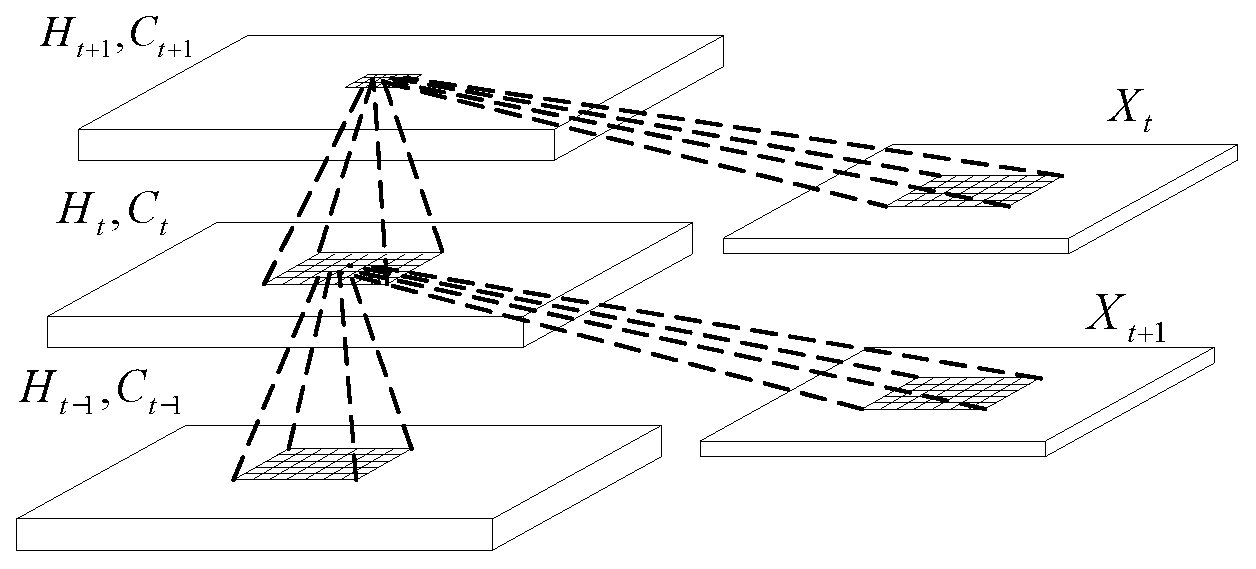
\includegraphics[width=0.8\columnwidth]{preliminaries_figs/ConvLSTM_model.eps}
		\caption{The inner structure of ConvLSMT network [ref]. 
        \label{fig:ConvLSTM_model}}
\end{figure}